\begin{frame}[fragile,shrink=5]{Symbolic form of large-deformation elasticity}
  Find displacement vector $\uu$ such that:
  \begin{equation*}
    \int_\Omega \nabla \vv \tcolon \Pi = 0,\quad \forall \vv
  \end{equation*}
  where
  \begin{align*}
    F   & = I - \nabla \uu                &  & \text{Deformation gradient}  \\
    E   & = (F^T F - I)/2                 &  & \text{Green-Lagrange tensor} \\
    S   & = \lambda (\trace E) I + 2\mu E &  & \text{Second Piola-Kirchoff tensor} \\
\uncover<2>{\alert{S}   & \alert{ = \lambda (J^2 - I) C^{-1} + \mu (I - C^{-1})}} & & \uncover<2>{\text{Neo-Hookean material, } (C = F^T F)} \\
    \Pi & = F \cdot S                     &  & \text{First Piola-Kirchoff tensor}
  \end{align*}
  \vspace{-0.8em}
\begin{pythoncode}
  def weak_form(u, du, v, dv):
    I = eye(3)                      # Identity tensor
    F = I - du                      # Deformation gradient
    E = (F.T*F - I)/2               # Green-Lagrange tensor
    S = lmbda*E.trace()*I + 2*mu*E  # Second Piola-Kirchoff tensor
    Pi = F * S                      # First Piola-Kirchoff tensor
    return dv.dot(Pi)
\end{pythoncode}
\end{frame}

\begin{frame}[fragile]{Manufactured solution}
  \begin{itemize}
  \item Choose a solution $\uu_{\text{exact}}$ with rich derivatives
  \begin{pythoncode}
  def solution(x,y,z, a,b,c):
    return Matrix([cos(x) * exp(y) * z + sin(z),
                   sin(x) * tanh(y) + x * cosh(z),
                   exp(x) * sinh(y) + y * log(1+z**2)])
  \end{pythoncode}
  \item Apply strong-form nonlinear differential operator symbolically
    to define
    \[ f(x,y,z) = \nabla\cdot \Pi(\nabla \uu_{\text{exact}}) \]
  \item Solve finite element problem for $\uu_h$
    \begin{equation*}
      \int_\Omega \nabla \vv \tcolon \Pi(\nabla \uu_h) = \int v\cdot f(x,y,z),\quad \forall \vv
    \end{equation*}
  \item Compute norms of $\uu_h - \uu_{\text{exact}}$.
  \end{itemize}
\end{frame}

\begin{frame}{Manufactured solution}
  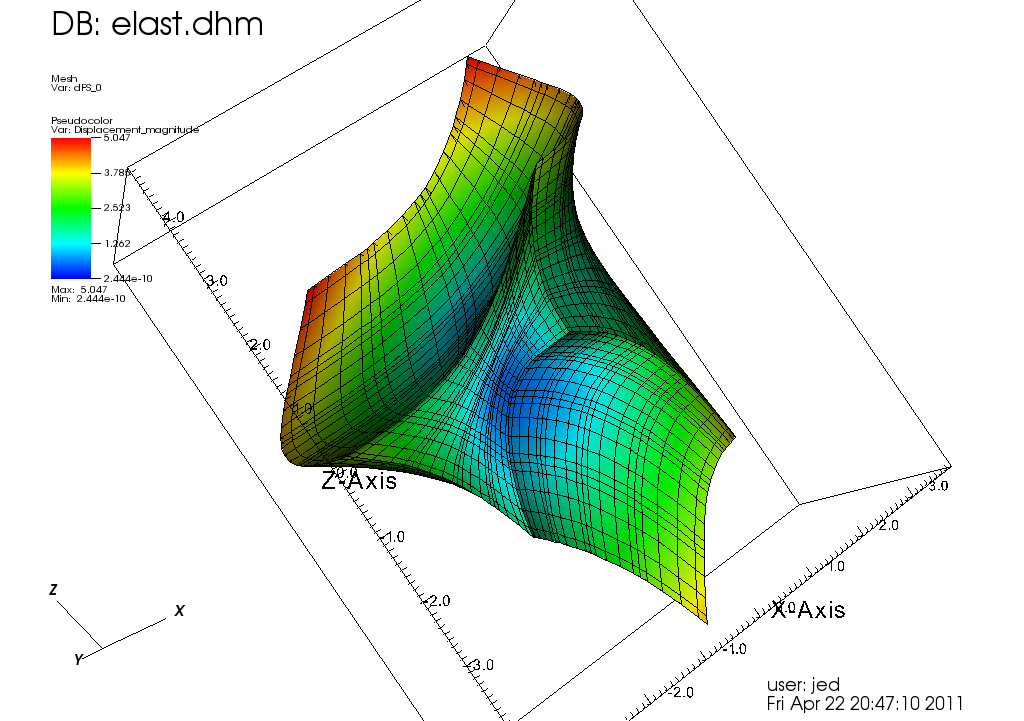
\includegraphics[width=\textwidth]{figures/elast-b4q5} \\
\end{frame}

\begin{frame}[shrink=30]{Convergence rates}
  \begin{tabular}{lrr rr rr rr rr}
    \toprule
    & & & \multicolumn{2}{c}{$\norm{\uu_h - \uu}_2$} & \multicolumn{2}{c}{$\norm{\uu_h - \uu}_\infty$}
    & \multicolumn{2}{c}{$\norm{\nabla\uu_h - \nabla\uu}_2$} & \multicolumn{2}{c}{$\norm{\nabla\uu_h - \nabla\uu}_\infty$} \\
    \cmidrule(r){4-5} \cmidrule(lr){6-7} \cmidrule(lr){8-9} \cmidrule(l){10-11}
    \multicolumn{2}{c}{Mesh} & \# Nodes & Error & \bigO & Error & \bigO & Error & \bigO & Error & \bigO \\
    \midrule % output below is generated with verif.py in this directory
$Q_1$ & $1^3$ & 8 & 1.79e+00 & --- & 6.50e-01 & --- & 3.70e+00 & --- & 1.08e+00 & --- \\
$Q_1$ & $2^3$ & 27 & 5.49e-01 & 1.71 & 3.40e-01 & 0.93 & 1.61e+00 & 1.20 & 6.92e-01 & 0.64 \\
$Q_1$ & $4^3$ & 125 & 1.53e-01 & 1.84 & 1.26e-01 & 1.43 & 8.01e-01 & 1.01 & 4.51e-01 & 0.62 \\
$Q_1$ & $8^3$ & 729 & 3.94e-02 & 1.96 & 3.73e-02 & 1.76 & 3.98e-01 & 1.01 & 2.81e-01 & 0.68 \\
$Q_1$ & $16^3$ & 4913 & 9.95e-03 & 1.99 & 1.01e-02 & 1.88 & 1.98e-01 & 1.01 & 1.57e-01 & 0.84 \\
$Q_1$ & $32^3$ & 35937 & 2.49e-03 & 2.00 & 2.61e-03 & 1.95 & 9.92e-02 & 1.00 & 8.32e-02 & 0.92\\
% \midrule
% $Q_2$ & $1^3$ & 27 & 2.44e-01 & --- & 1.82e-01 & --- & 9.48e-01 & --- & 4.60e-01 & --- \\
% $Q_2$ & $2^3$ & 125 & 3.71e-02 & 2.72 & 4.47e-02 & 2.03 & 2.86e-01 & 1.73 & 1.54e-01 & 1.58 \\
% $Q_2$ & $4^3$ & 729 & 4.48e-03 & 3.05 & 6.23e-03 & 2.84 & 6.94e-02 & 2.04 & 4.34e-02 & 1.83 \\
% $Q_2$ & $8^3$ & 4913 & 5.60e-04 & 3.00 & 9.31e-04 & 2.74 & 1.74e-02 & 2.00 & 1.29e-02 & 1.75 \\
% $Q_2$ & $16^3$ & 35937 & 7.01e-05 & 3.00 & 1.23e-04 & 2.92 & 4.34e-03 & 2.00 & 3.52e-03 & 1.87\\
\midrule
$Q_3$ & $1^3$ & 64 & 4.14e-02 & --- & 2.71e-02 & --- & 2.90e-01 & --- & 1.63e-01 & --- \\
$Q_3$ & $2^3$ & 343 & 2.06e-03 & 4.33 & 2.06e-03 & 3.72 & 2.39e-02 & 3.60 & 1.14e-02 & 3.84 \\
$Q_3$ & $4^3$ & 2197 & 1.81e-04 & 3.51 & 2.06e-04 & 3.32 & 4.23e-03 & 2.50 & 2.88e-03 & 1.98 \\
$Q_3$ & $8^3$ & 15625 & 1.22e-05 & 3.89 & 1.87e-05 & 3.46 & 5.79e-04 & 2.87 & 5.84e-04 & 2.30\\
\midrule
$Q_5$ & $1^3$ & 216 & 3.76e-03 & --- & 2.90e-03 & --- & 4.69e-02 & --- & 3.16e-02 & --- \\
$Q_5$ & $2^3$ & 1331 & 7.58e-05 & 5.63 & 5.92e-05 & 5.61 & 1.62e-03 & 4.86 & 1.05e-03 & 4.91 \\
$Q_5$ & $4^3$ & 9261 & 7.33e-07 & 6.69 & 6.61e-07 & 6.48 & 2.59e-05 & 5.97 & 1.76e-05 & 5.90\\
% \midrule
% $Q_7$ & $1^3$ & 512 & 4.46e-04 & --- & 3.59e-04 & --- & 8.15e-03 & --- & 5.83e-03 & --- \\
% $Q_7$ & $2^3$ & 3375 & 2.95e-06 & 7.24 & 2.95e-06 & 6.93 & 8.21e-05 & 6.63 & 6.05e-05 & 6.59 \\
% $Q_7$ & $4^3$ & 24389 & 7.65e-09 & 8.59 & 1.07e-08 & 8.11 & 4.09e-07 & 7.65 & 3.95e-07 & 7.26\\
\midrule
$Q_9$ & $1^3$ & 1000 & 5.81e-05 & --- & 5.04e-05 & --- & 1.42e-03 & --- & 1.05e-03 & --- \\
$Q_9$ & $2^3$ & 6859 & 6.27e-08 & 9.86 & 7.59e-08 & 9.38 & 1.63e-06 & 9.77 & 1.60e-06 & 9.36 \\
\bottomrule
  \end{tabular}
\end{frame}
